%% Standalone lecture -- build with:  pdflatex -shell-escape mcmc
%% Shared preamble for standalone lecture files.
%%
%% Every lecture begins with %% Shared preamble for standalone lecture files.
%%
%% Every lecture begins with %% Shared preamble for standalone lecture files.
%%
%% Every lecture begins with \input{preamble} and is compiled on its own:
%%     pdflatex -shell-escape <lecture>
%% There is no master lectures.tex any more -- the list of lectures lives in
%% lectures.yaml and is read by the build scripts.

\documentclass[25pt,landscape,footrule]{foils}
\input{macros_gen}
\backgroundsetup{contents={}}

\usepackage{stmaryrd}
\usepackage{ifthen}
\usepackage{pdf14}

% Every figure lives in this course's lectures/figures (consolidated
% 2026-10-08).  Do not add other courses' folders back: when a name exists in
% several folders LaTeX silently takes the first, which mixed old and new
% frames of the same animation.  A missing figure should be a build error.
\graphicspath{{figures/}{../lectures/figures/}}

\date{}

\newcounter{lessoncnt}
\newcommand{\lesson}[1]{\setcounter{page}{1}%
\section{Mathematics of Machine Learning\\%
\vfill
\textcolor{red}{\textit{#1}}
\vfill}}
 and is compiled on its own:
%%     pdflatex -shell-escape <lecture>
%% There is no master lectures.tex any more -- the list of lectures lives in
%% lectures.yaml and is read by the build scripts.

\documentclass[25pt,landscape,footrule]{foils}
%\usepackage[compat2,pdftex]{geometry}
\usepackage[pdftex]{geometry}
\geometry{headsep=-2.5ex,hscale=0.9,bmargin=2.5cm,tmargin=1cm,textwidth=25cm}
\usepackage[pdftex]{xcolor}
\usepackage{pause}
\usepackage{background}
%\usepackage[color=white]{background}
\usepackage{listings}
\usepackage{graphicx}
\usepackage{epsfig}
\usepackage{epstopdf}
\usepackage{bm}
\usepackage{amssymb}
\usepackage{amsfonts}
\usepackage{marvosym}
\usepackage{cite}
\usepackage{pifont}
\usepackage[english]{babel}
\usepackage{amsmath}
\usepackage{amsfonts}
\usepackage{rotating}
\usepackage{listings}
\usepackage{pp4slide}
%\usepackage{hyperref}
\usepackage{pp4link}
\usepackage{fancyvrb}
\usepackage{multido}
\usepackage{calc}
\usepackage{mleftright}
\mleftright % Redefines \left to \mleft and \right to \mright



\thinmuskip=1mu

\newcommand{\bigstrut}{\rule[-0.5\baselineskip]{0pt}{1.2\baselineskip}}
\renewcommand{\ttdefault}{pcr}

\newcommand{\squeeze}{\setlength{\itemsep}{-2pt}}
%\renewcommand{\familydefault}{cmr}
%\renewcommand{\labelitemii}{\textcolor{green}{$\star$}}
\newcommand{\tick}{{\large \ding{51}}}
\newcommand{\cross}{{\large \ding{55}}}
%\DeclareMathAlphabet{\mat}{OT1}{cmss}{bx}{n}
\DeclareMathAlphabet{\mat}{U}{eur}{b}{n}
\newcommand{\figs}{/home/apb/figures}
\newcommand{\stimes}{{\scriptstyle \times}}
\newcommand{\tr}{\textsf{T}}
\newcommand{\e}[1]{{\rm e}^{#1}}
\newcommand{\E}[1]{{\rm e}^{{\displaystyle #1}}}
\newcommand{\av}[2][]{\mathbb{E}_{#1}\left[ #2 \right]}
\newcommand{\Var}[1]{\mathbb{V}\mathrm{ar}\left( #1 \right)}
\newcommand{\pred}[1]{\left\llbracket { \small #1} \right\rrbracket}
\newcommand{\logg}[1]{\log\left( #1 \right)}
\newcommand{\logtwo}[1]{\log_2\left( #1 \right)}
\newcommand{\bra}[1]{\left( #1 \right)}
\newcommand{\prob}[1]{\mathbb{P}\left( #1 \right)}
\newcommand{\Prob}[1]{\mathbb{P}\left( #1 \right)}
\newcommand{\Step}{\mathop{\mat{\Theta}}}
\newcommand\diag{\mathop{\mathrm{diag}}}
\newcommand{\grad}{\bm{\nabla}}
\newcommand{\gradx}{\bm{\nabla}_{\!\!\scriptscriptstyle \bm{x}}}
\newcommand{\gradw}{\bm{\nabla}_{\!\!\scriptscriptstyle \bm{w}}}
\newcommand{\dd}{\mathrm{d}}
\newcommand{\ii}{\mathrm{i}}
\newcommand{\data}{\mathcal{D}}
\newcommand{\class}{\mathcal{C}}
\newcommand{\hypo}{\mathcal{H}}
\newcommand{\indep}{\perp \!\!\!\! \perp}
\newcommand{\pd}[3][\,]{\frac{\partial^{#1}{#2}}{\partial\,{#3}}}
\newcommand{\normal}[1]{\mathcal{N}\!\left( #1 \right)}
\newcommand{\Dist}[2][Binom]{\mathrm{#1}\left( \strut {#2} \right)}
\newcommand{\brackets}[1]{\!\left( #1 \right)}
\newcommand{\KL}[2]{\mathop{\mathrm{KL}}\left(#1 \big\| #2\right)}
\newcommand{\argmax}{\mathop{\mathrm{argmax}}}
\newcommand{\argmin}{\mathop{\mathrm{argmin}}}
\newcommand{\margin}{\Delta}
\lstnewenvironment{matlab}[1][frame=TB]{\lstset{#1}}{}       
%\renewcommand{\emph}[1]{\textcolor{red}{\textbf{#1}}}
\newcommand{\myskip}[1]{}
\newcommand\mycom[2]{\genfrac{}{}{0pt}{}{#1}{#2}}
\newcommand{\jl}{\lstinline[basicstyle=\ttfamily\color{DarkGreen},%
 keywordstyle=\bfseries\ttfamily\color{DarkGreen}]}
\definecolor{EmphColor}{rgb}{0.0,0.0,1.0}
\renewcommand{\emph}[1]{{\color{EmphColor}\textbf{#1}}}
\newcommand{\len}[1]{\| #1 \|}
\newcommand{\inner}[2]{\left\langle {#1}, {#2}\right\rangle}
\newenvironment{psmallmatrix}{\left(\begin{smallmatrix}}{\end{smallmatrix}\right)}
  

\definecolor{DarkGreen}{rgb}{0,0.5,0}
\definecolor{DarkRed}{rgb}{0,0,0.5}
\definecolor{HighLight}{rgb}{1,0,0}     % yellow
\definecolor{TextColor}{rgb}{0.0,0.1,0.1}     % white
\definecolor{TwoColor}{rgb}{0.0,0.5,0.1}      % used for switching colors

\definecolor{HeadLineColor}{rgb}{1.0,0.0,0.0} % cyan
\definecolor{SpecialColor}{rgb}{0.53,0.81,1.0}
\renewcommand{\normalcolor}{\color{HeadLineColor}}

\pausecolors{TwoColor}{TextColor}{HighLight}
\pausecolors{EmphColor}{TextColor}{EmphColor}
\pausecolors{DarkGreen}{DarkGreen}{DarkRed}
\pausecolors{SpecialColor}{white}{HighLight}

\newenvironment{PauseHighLight}{\color{TwoColor}\pausehighlight}{}
\newcommand{\multipdf}[2][width=\linewidth]{\multiinclude[pause=\pauselevel{:+0}\pause,format=pdf,graphics={#1}]{#2}}

\lstdefinelanguage{pseudo}
 {keywords={all,and,begin,break,continue,do,else,elseif,%
     end,endif,endfor,endwhile,%
     exit,false,for,forall,goto,if,%
     or,return,then,true,to,repeat,until,while},%
  comment=[s]{/*}{*/},%
  morecomment=[l]//,%
  morestring=[d]"%
 }[keywords,comments,strings]


\lstloadlanguages{Java,pseudo,Python}
\lstset{
  basicstyle=\footnotesize\ttfamily\color{DarkGreen},
  keywordstyle=\bfseries\footnotesize\ttfamily\color{DarkGreen},
  commentstyle=\footnotesize\it\rmfamily\color{blue},
  language=Java,
  showstringspaces=false
  }


\lstnewenvironment{pseudo}[1][]{\lstset{language=pseudo,mathescape,literate={:=}{{$\gets$}}2 {!}{{$\neg$}}1 {!=}{{\!\!$\neq$\,\,}}2 {<=}{{\!\!$\leq$\,\,}}2 {>=}{{\!\!$\geq$\,\,}}2,escapechar=\#,#1}}{}
\lstnewenvironment{java}[1][]{\lstset{escapechar=\$,#1}}{}
% Python code: the language setting makes # comments use commentstyle.
% Comments stay monospaced: the default italic roman letter-spaces badly
% on listings' fixed columns.
\lstnewenvironment{python}[1][frame=TB]{\lstset{language=Python,
    commentstyle=\footnotesize\ttfamily\color{blue},#1}}{}

\MyLogo{}
%\Restriction{}
%\rightfooter{\hyperlink{overview}{$\square$}}

\newcommand{\keywords}[1]{\vfill{\noindent\it #1}}

\newcounter{outlineitem}
\setcounter{outlineitem}{0}
\newcommand{\outlineitem}[2]{\item%
  \def\targ{\value{emumi}}%
  \ifnum\value{enumi}=\value{outlineitem}%
  \color{HighLight}\textbf{#1}\toptarget{#2}\color{TextColor}%
   \else\toplink{#2}{#1}\fi
}
\color{TwoColor}


%-- Instead of writing \section we want the file structured by \section.
\newcommand{\section}[2][0]{\foilhead[#1cm]{#2}}

%-- Write each page into a \begin{slide} -- \end{slide} environment.
\newenvironment{slide}{}{\pauselevel{=1}}

\MyLogo{\pauselevel{=1}\Acrobatmenu{GoBack}{%
  \color{TextColor}{Adam Pr\"ugel-Bennett}} \hspace{2cm}
  % Clicking on the name steps one slide back.
  \toplink{firstoutline}{\color{red}Mathematics of Machine
    Learning}%
  \hspace{2cm}
  \texttt{//ecs-vlc.github.io/aice3001/}
  %Clicking on the date jumps to the last page, which should be the
  %table of contents.
  \rightfooter{\Acrobatmenu{LastPage}{\qquad%
  \textsf{\color{TextColor}\tiny\thepage}}}% page number
  % Clicking on the page number steps one slide back.
}
\raggedright
\newcommand{\Outline}{}

\newcommand{\pb}{\pausebuild \color{TwoColor}}
\newcommand{\pauseb}{\pauselevel{build, highlight}\pause}
\newcommand{\hl}[1]{\pauselevel{=1, highlight =1 :1, highlight =#1 :#1}\pause}
\newcommand{\hll}{\pauselevel{=1, highlight =1 :1}\pause}
\newcommand{\pauseh}{\pauselevel{highlight}\pause}
\newcommand{\nhl}[1]{\textcolor{TextColor}{#1}}
\newcommand{\mypl}[1]{\pauselevel{=#1 :#1}\pause}
\input supp-pdf.tex
\DeclareGraphicsRule{*}{mps}{*}{}
\usepackage{mpmulti}
%\leftheader{}
\rightheader{} % no more page numbers on top right


\hypersetup{pdftitle={ECS Lectures},pdfsubject={Machine Learning}
pdfauthor={Adam Prugel-Bennett},pdfkeywords={machine learning},
pdfpagemode={FullScreen},
bookmarksopen=false,
hypertexnames=false,pdfstartview={FitV},colorlinks,linkcolor={blue},
citecolor={green},urlcolor={blue}}



\newcommand\bluepage{
\clearpage
\renewcommand\normalcolor{\color{yellow}}
\pagecolor{blue}
\renewcommand\Black{\color{white}}
\color{white}
\hypersetup{colorlinks=true}
}

\newcommand\whitepage{
\clearpage
\renewcommand\normalcolor{\color{black}}
\pagecolor{white}
\renewcommand\Black{\color{black}}
\color{black}
\hypersetup{colorlinks=true}
}

\whitepage
\setlength{\unitlength}{1mm}

\newenvironment{leftImage}[2][0.3]{%
\begin{minipage}{#1\linewidth}
  \includegraphics[width=\linewidth]{#2}
\end{minipage}\hfill
\begin{minipage}{0.92\linewidth - #1\linewidth}}%
{\end{minipage}}

\newenvironment{rightImage}[2][0.3]{%
\newcommand{\foot}{\begin{minipage}{#1\linewidth}\includegraphics[width=0.98\linewidth]{#2}\end{minipage}}%
\begin{minipage}{0.95\linewidth - #1\linewidth}\raggedright }{\end{minipage}\hfill\foot}


%%% Local Variables: 
%%% mode: latex
%%% TeX-master: t
%%% End: 

\backgroundsetup{contents={}}

\usepackage{stmaryrd}
\usepackage{ifthen}
\usepackage{pdf14}

% Every figure lives in this course's lectures/figures (consolidated
% 2026-10-08).  Do not add other courses' folders back: when a name exists in
% several folders LaTeX silently takes the first, which mixed old and new
% frames of the same animation.  A missing figure should be a build error.
\graphicspath{{figures/}{../lectures/figures/}}

\date{}

\newcounter{lessoncnt}
\newcommand{\lesson}[1]{\setcounter{page}{1}%
\section{Mathematics of Machine Learning\\%
\vfill
\textcolor{red}{\textit{#1}}
\vfill}}
 and is compiled on its own:
%%     pdflatex -shell-escape <lecture>
%% There is no master lectures.tex any more -- the list of lectures lives in
%% lectures.yaml and is read by the build scripts.

\documentclass[25pt,landscape,footrule]{foils}
%\usepackage[compat2,pdftex]{geometry}
\usepackage[pdftex]{geometry}
\geometry{headsep=-2.5ex,hscale=0.9,bmargin=2.5cm,tmargin=1cm,textwidth=25cm}
\usepackage[pdftex]{xcolor}
\usepackage{pause}
\usepackage{background}
%\usepackage[color=white]{background}
\usepackage{listings}
\usepackage{graphicx}
\usepackage{epsfig}
\usepackage{epstopdf}
\usepackage{bm}
\usepackage{amssymb}
\usepackage{amsfonts}
\usepackage{marvosym}
\usepackage{cite}
\usepackage{pifont}
\usepackage[english]{babel}
\usepackage{amsmath}
\usepackage{amsfonts}
\usepackage{rotating}
\usepackage{listings}
\usepackage{pp4slide}
%\usepackage{hyperref}
\usepackage{pp4link}
\usepackage{fancyvrb}
\usepackage{multido}
\usepackage{calc}
\usepackage{mleftright}
\mleftright % Redefines \left to \mleft and \right to \mright



\thinmuskip=1mu

\newcommand{\bigstrut}{\rule[-0.5\baselineskip]{0pt}{1.2\baselineskip}}
\renewcommand{\ttdefault}{pcr}

\newcommand{\squeeze}{\setlength{\itemsep}{-2pt}}
%\renewcommand{\familydefault}{cmr}
%\renewcommand{\labelitemii}{\textcolor{green}{$\star$}}
\newcommand{\tick}{{\large \ding{51}}}
\newcommand{\cross}{{\large \ding{55}}}
%\DeclareMathAlphabet{\mat}{OT1}{cmss}{bx}{n}
\DeclareMathAlphabet{\mat}{U}{eur}{b}{n}
\newcommand{\figs}{/home/apb/figures}
\newcommand{\stimes}{{\scriptstyle \times}}
\newcommand{\tr}{\textsf{T}}
\newcommand{\e}[1]{{\rm e}^{#1}}
\newcommand{\E}[1]{{\rm e}^{{\displaystyle #1}}}
\newcommand{\av}[2][]{\mathbb{E}_{#1}\left[ #2 \right]}
\newcommand{\Var}[1]{\mathbb{V}\mathrm{ar}\left( #1 \right)}
\newcommand{\pred}[1]{\left\llbracket { \small #1} \right\rrbracket}
\newcommand{\logg}[1]{\log\left( #1 \right)}
\newcommand{\logtwo}[1]{\log_2\left( #1 \right)}
\newcommand{\bra}[1]{\left( #1 \right)}
\newcommand{\prob}[1]{\mathbb{P}\left( #1 \right)}
\newcommand{\Prob}[1]{\mathbb{P}\left( #1 \right)}
\newcommand{\Step}{\mathop{\mat{\Theta}}}
\newcommand\diag{\mathop{\mathrm{diag}}}
\newcommand{\grad}{\bm{\nabla}}
\newcommand{\gradx}{\bm{\nabla}_{\!\!\scriptscriptstyle \bm{x}}}
\newcommand{\gradw}{\bm{\nabla}_{\!\!\scriptscriptstyle \bm{w}}}
\newcommand{\dd}{\mathrm{d}}
\newcommand{\ii}{\mathrm{i}}
\newcommand{\data}{\mathcal{D}}
\newcommand{\class}{\mathcal{C}}
\newcommand{\hypo}{\mathcal{H}}
\newcommand{\indep}{\perp \!\!\!\! \perp}
\newcommand{\pd}[3][\,]{\frac{\partial^{#1}{#2}}{\partial\,{#3}}}
\newcommand{\normal}[1]{\mathcal{N}\!\left( #1 \right)}
\newcommand{\Dist}[2][Binom]{\mathrm{#1}\left( \strut {#2} \right)}
\newcommand{\brackets}[1]{\!\left( #1 \right)}
\newcommand{\KL}[2]{\mathop{\mathrm{KL}}\left(#1 \big\| #2\right)}
\newcommand{\argmax}{\mathop{\mathrm{argmax}}}
\newcommand{\argmin}{\mathop{\mathrm{argmin}}}
\newcommand{\margin}{\Delta}
\lstnewenvironment{matlab}[1][frame=TB]{\lstset{#1}}{}       
%\renewcommand{\emph}[1]{\textcolor{red}{\textbf{#1}}}
\newcommand{\myskip}[1]{}
\newcommand\mycom[2]{\genfrac{}{}{0pt}{}{#1}{#2}}
\newcommand{\jl}{\lstinline[basicstyle=\ttfamily\color{DarkGreen},%
 keywordstyle=\bfseries\ttfamily\color{DarkGreen}]}
\definecolor{EmphColor}{rgb}{0.0,0.0,1.0}
\renewcommand{\emph}[1]{{\color{EmphColor}\textbf{#1}}}
\newcommand{\len}[1]{\| #1 \|}
\newcommand{\inner}[2]{\left\langle {#1}, {#2}\right\rangle}
\newenvironment{psmallmatrix}{\left(\begin{smallmatrix}}{\end{smallmatrix}\right)}
  

\definecolor{DarkGreen}{rgb}{0,0.5,0}
\definecolor{DarkRed}{rgb}{0,0,0.5}
\definecolor{HighLight}{rgb}{1,0,0}     % yellow
\definecolor{TextColor}{rgb}{0.0,0.1,0.1}     % white
\definecolor{TwoColor}{rgb}{0.0,0.5,0.1}      % used for switching colors

\definecolor{HeadLineColor}{rgb}{1.0,0.0,0.0} % cyan
\definecolor{SpecialColor}{rgb}{0.53,0.81,1.0}
\renewcommand{\normalcolor}{\color{HeadLineColor}}

\pausecolors{TwoColor}{TextColor}{HighLight}
\pausecolors{EmphColor}{TextColor}{EmphColor}
\pausecolors{DarkGreen}{DarkGreen}{DarkRed}
\pausecolors{SpecialColor}{white}{HighLight}

\newenvironment{PauseHighLight}{\color{TwoColor}\pausehighlight}{}
\newcommand{\multipdf}[2][width=\linewidth]{\multiinclude[pause=\pauselevel{:+0}\pause,format=pdf,graphics={#1}]{#2}}

\lstdefinelanguage{pseudo}
 {keywords={all,and,begin,break,continue,do,else,elseif,%
     end,endif,endfor,endwhile,%
     exit,false,for,forall,goto,if,%
     or,return,then,true,to,repeat,until,while},%
  comment=[s]{/*}{*/},%
  morecomment=[l]//,%
  morestring=[d]"%
 }[keywords,comments,strings]


\lstloadlanguages{Java,pseudo,Python}
\lstset{
  basicstyle=\footnotesize\ttfamily\color{DarkGreen},
  keywordstyle=\bfseries\footnotesize\ttfamily\color{DarkGreen},
  commentstyle=\footnotesize\it\rmfamily\color{blue},
  language=Java,
  showstringspaces=false
  }


\lstnewenvironment{pseudo}[1][]{\lstset{language=pseudo,mathescape,literate={:=}{{$\gets$}}2 {!}{{$\neg$}}1 {!=}{{\!\!$\neq$\,\,}}2 {<=}{{\!\!$\leq$\,\,}}2 {>=}{{\!\!$\geq$\,\,}}2,escapechar=\#,#1}}{}
\lstnewenvironment{java}[1][]{\lstset{escapechar=\$,#1}}{}
% Python code: the language setting makes # comments use commentstyle.
% Comments stay monospaced: the default italic roman letter-spaces badly
% on listings' fixed columns.
\lstnewenvironment{python}[1][frame=TB]{\lstset{language=Python,
    commentstyle=\footnotesize\ttfamily\color{blue},#1}}{}

\MyLogo{}
%\Restriction{}
%\rightfooter{\hyperlink{overview}{$\square$}}

\newcommand{\keywords}[1]{\vfill{\noindent\it #1}}

\newcounter{outlineitem}
\setcounter{outlineitem}{0}
\newcommand{\outlineitem}[2]{\item%
  \def\targ{\value{emumi}}%
  \ifnum\value{enumi}=\value{outlineitem}%
  \color{HighLight}\textbf{#1}\toptarget{#2}\color{TextColor}%
   \else\toplink{#2}{#1}\fi
}
\color{TwoColor}


%-- Instead of writing \section we want the file structured by \section.
\newcommand{\section}[2][0]{\foilhead[#1cm]{#2}}

%-- Write each page into a \begin{slide} -- \end{slide} environment.
\newenvironment{slide}{}{\pauselevel{=1}}

\MyLogo{\pauselevel{=1}\Acrobatmenu{GoBack}{%
  \color{TextColor}{Adam Pr\"ugel-Bennett}} \hspace{2cm}
  % Clicking on the name steps one slide back.
  \toplink{firstoutline}{\color{red}Mathematics of Machine
    Learning}%
  \hspace{2cm}
  \texttt{//ecs-vlc.github.io/aice3001/}
  %Clicking on the date jumps to the last page, which should be the
  %table of contents.
  \rightfooter{\Acrobatmenu{LastPage}{\qquad%
  \textsf{\color{TextColor}\tiny\thepage}}}% page number
  % Clicking on the page number steps one slide back.
}
\raggedright
\newcommand{\Outline}{}

\newcommand{\pb}{\pausebuild \color{TwoColor}}
\newcommand{\pauseb}{\pauselevel{build, highlight}\pause}
\newcommand{\hl}[1]{\pauselevel{=1, highlight =1 :1, highlight =#1 :#1}\pause}
\newcommand{\hll}{\pauselevel{=1, highlight =1 :1}\pause}
\newcommand{\pauseh}{\pauselevel{highlight}\pause}
\newcommand{\nhl}[1]{\textcolor{TextColor}{#1}}
\newcommand{\mypl}[1]{\pauselevel{=#1 :#1}\pause}
\input supp-pdf.tex
\DeclareGraphicsRule{*}{mps}{*}{}
\usepackage{mpmulti}
%\leftheader{}
\rightheader{} % no more page numbers on top right


\hypersetup{pdftitle={ECS Lectures},pdfsubject={Machine Learning}
pdfauthor={Adam Prugel-Bennett},pdfkeywords={machine learning},
pdfpagemode={FullScreen},
bookmarksopen=false,
hypertexnames=false,pdfstartview={FitV},colorlinks,linkcolor={blue},
citecolor={green},urlcolor={blue}}



\newcommand\bluepage{
\clearpage
\renewcommand\normalcolor{\color{yellow}}
\pagecolor{blue}
\renewcommand\Black{\color{white}}
\color{white}
\hypersetup{colorlinks=true}
}

\newcommand\whitepage{
\clearpage
\renewcommand\normalcolor{\color{black}}
\pagecolor{white}
\renewcommand\Black{\color{black}}
\color{black}
\hypersetup{colorlinks=true}
}

\whitepage
\setlength{\unitlength}{1mm}

\newenvironment{leftImage}[2][0.3]{%
\begin{minipage}{#1\linewidth}
  \includegraphics[width=\linewidth]{#2}
\end{minipage}\hfill
\begin{minipage}{0.92\linewidth - #1\linewidth}}%
{\end{minipage}}

\newenvironment{rightImage}[2][0.3]{%
\newcommand{\foot}{\begin{minipage}{#1\linewidth}\includegraphics[width=0.98\linewidth]{#2}\end{minipage}}%
\begin{minipage}{0.95\linewidth - #1\linewidth}\raggedright }{\end{minipage}\hfill\foot}


%%% Local Variables: 
%%% mode: latex
%%% TeX-master: t
%%% End: 

\backgroundsetup{contents={}}

\usepackage{stmaryrd}
\usepackage{ifthen}
\usepackage{pdf14}

% Every figure lives in this course's lectures/figures (consolidated
% 2026-10-08).  Do not add other courses' folders back: when a name exists in
% several folders LaTeX silently takes the first, which mixed old and new
% frames of the same animation.  A missing figure should be a build error.
\graphicspath{{figures/}{../lectures/figures/}}

\date{}

\newcounter{lessoncnt}
\newcommand{\lesson}[1]{\setcounter{page}{1}%
\section{Mathematics of Machine Learning\\%
\vfill
\textcolor{red}{\textit{#1}}
\vfill}}


\begin{document}

\lesson{MCMC}
\vspace{-1cm}
\begin{center}
  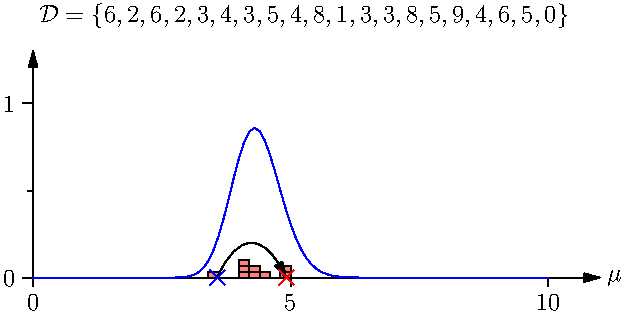
\includegraphics[height=10cm]{trafficMCMC-19}
\end{center}
\keywords{Monte Carlo methods, MCMC, Metropolis-Hastings, Gibbs sampling, Hamiltonian Monte Carlo, Convergence diagnostics}
%%%%%%%%%%%%%%%%%%%%%%% Next Slide %%%%%%%%%%%%%%%%%%%%%%%
\renewcommand{\Outline}{%
\begin{slide}
\section[1]{Outline}

\begin{minipage}{10cm}\raggedright
  \begin{enumerate}\squeeze
    \outlineitem{Monte Carlo}{mc}
    \outlineitem{MCMC}{mcmc}
    \outlineitem{Modern MCMC}{modern}
  \end{enumerate}
\end{minipage}\hfill
\begin{minipage}{12cm}
  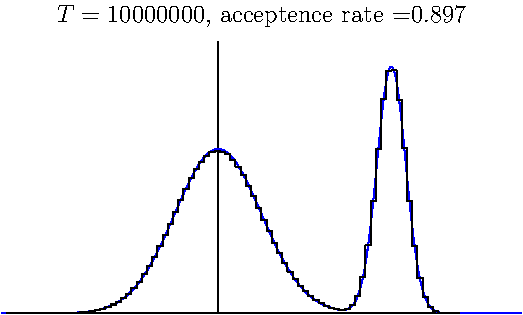
\includegraphics[width=12cm]{mcmc5}
\end{minipage}
\end{slide}
\addtocounter{outlineitem}{1}
}

\setcounter{outlineitem}{1}
\Outline % Monte Carlo
\toptarget{firstoutline}
%%%%%%%%%%%%%%%%%%%%%%% Next Slide %%%%%%%%%%%%%%%%%%%%%%%

\begin{slide}
\section[-2]{Bayesian Inference Gets Hard}

\begin{PauseHighLight}
  \begin{itemize}
  \item With a simple likelihood (normal, binomial, Poisson,
    multinomial) a conjugate prior gives a posterior of the same
    form\pause
  \item Most real models (e.g.\ hierarchical models) have no conjugate
    prior\pause
  \item We can still compute the top of Bayes' rule
    \begin{align*}
      f\brackets{\bm{\theta}|\data} = \frac{f\brackets{\data|\bm{\theta}} \,
      f\brackets{\bm{\theta}}}{ f\brackets{\data} }\pause
    \end{align*}
  \item But the evidence $f(\data)$ is an integral over all
    $\bm{\theta}$, which we usually cannot do\pause{}: this lecture
    shows how to draw samples from the posterior anyway\pauseb
  \end{itemize}
\end{PauseHighLight}

\end{slide}

%%%%%%%%%%%%%%%%%%%%%%% Next Slide %%%%%%%%%%%%%%%%%%%%%%%

\begin{slide}
\section{Histograms, Samples and Means}

\begin{PauseHighLight}
  \begin{itemize}
  \item We could represent our posterior as a histogram, although for
    multivariate distributions (i.e. when we are modelling more than one
    variable) a histogram can be unwieldy\pause
  \item A sample from the posterior distribution is often sufficient
    e.g. in a topic model of documents a typical set of topics is what we
    are after\pause
  \item However, when samples vary a lot, often the most useful quantities
    are expectations, e.g.
    \begin{align*}
      &\av{\bm{\Theta}} & &\av{\Theta_i^2}-\av{\Theta_i}^2 \\
      &\av{\Theta_i\,\Theta_j} - \av{\Theta_i}\,\av{\Theta_j}
      && \av{\bm{\Theta}\,\bm{\Theta}^\tr} -\av{\bm{\Theta}}\,\av{\bm{\Theta}}^\tr\pause
    \end{align*}
  \end{itemize}
\end{PauseHighLight}

\end{slide}

%%%%%%%%%%%%%%%%%%%%%%% Next Slide %%%%%%%%%%%%%%%%%%%%%%%

\begin{slide}
\section[-2]{Sample Estimation}

\pb\pause\pauselevel{=1}
\begin{itemize}
\item If we can draw independent samples (aka \emph{deviates} or
  \emph{variates}), $\bm{\Theta}_i$, from our posterior distribution then we can
  obtain an estimate of our expectation
  \begin{align*}
    \av{g(\bm{\Theta})} \approx \frac{1}{n} \sum_{i=1}^n g(\bm{\Theta}_i)\pauseh
  \end{align*}
\item Provided our posterior distribution is well behaved (the
  variance of $g(\bm{\Theta})$ is finite) the error in our estimate
  will drop off as $1/\sqrt{n}$\pauseh
  \begin{center}
    \multipdf[width=\linewidth]{wellBehaved}\pause   
  \end{center}
\end{itemize}

\end{slide}

%%%%%%%%%%%%%%%%%%%%%%% Next Slide %%%%%%%%%%%%%%%%%%%%%%%

\begin{slide}
\section[-2]{Drawing Random Samples}

\pb
\begin{itemize}
\item Computing with (pseudo) random samples drawn from a
  distribution is known as \emph{Monte Carlo}\pauseh
\item For some very simple distributions we can use the \emph{transformation
  methods} to transform a uniform distribution\pauseh
\end{itemize}
\begin{center}
  \multipdf[width=\linewidth]{exponentialDeviates}\pause
\end{center}

\end{slide}

%%%%%%%%%%%%%%%%%%%%%%% Next Slide %%%%%%%%%%%%%%%%%%%%%%%

\begin{slide}
\section[-1]{Rejection Method}

\begin{PauseHighLight}
  \begin{itemize}
  \item The transformation method only works when we can easily compute
    the inverse \textit{cumulative distribution function} (CDF)\pause
  \item The \emph{rejection method} draws $Y$ from a density $g_Y$ with
    $c\,g_Y(x)\geq f_X(x)$ for all $x$, and accepts it with probability
    $f_X(Y)/(c\,g_Y(Y))$\pause
  \item A deviate is accepted with probability $1/c$, so on average
    we need $c$ tries for each deviate\pause
  \item Very general, but for complicated or multivariate distributions
    it is hard to find a good $g_Y$\pause{}, and $c$ can be enormous (it
    typically grows exponentially with the dimension)\pauseb
  \end{itemize}
\end{PauseHighLight}

\end{slide}

%%%%%%%%%%%%%%%%%%%%%%% Next Slide %%%%%%%%%%%%%%%%%%%%%%%

\begin{slide}
\section{Drawing Normal Deviates}

\pause
\pb
\pauselevel{=1}
\begin{center}
  \multipdf[width=\linewidth]{rejectionSampling}\pause
\end{center}

\end{slide}

%%%%%%%%%%%%%%%%%%%%%%% Next Slide %%%%%%%%%%%%%%%%%%%%%%%
\Outline % MCMC
%%%%%%%%%%%%%%%%%%%%%%% Next Slide %%%%%%%%%%%%%%%%%%%%%%%

\begin{slide}
\section[-1]{Detailed Balance}

\begin{PauseHighLight}
  \begin{itemize}
  \item Suppose we have a set of states $\mathcal{S}$ and want to draw
    samples from a probability distribution $\bm{\pi} = (\pi_i | i \in
    \mathcal{S})$\pause
  \item We invent a dynamical system with a transition probability $M_{ij}$ from state $j$ to
    state $i$ such that
    \begin{align*}
      M_{ij} \, \pi_j = M_{ji} \pi_i
    \end{align*}
  \item This is known as \emph{detailed balance}\pause
  \item Summing both sides over $j$ (using $\sum_j M_{ji}=1$: from $i$
    we must go somewhere)
    \begin{align*}
      \sum_{j} M_{ij}\,\pi_j &= \sum_{j} M_{ji}\,\pi_i \pause = \pi_i\pauseb
      &
        \mat{M} \bm{\pi} = \bm{\pi}\pauseb
    \end{align*}
  \end{itemize}
\end{PauseHighLight}

\end{slide}

%%%%%%%%%%%%%%%%%%%%%%% Next Slide %%%%%%%%%%%%%%%%%%%%%%%

\begin{slide}
\section[-2]{Convergence of MCMC}

\begin{PauseHighLight}
  \begin{itemize}
  \item Start from a probability vector $\bm{p}(0) = \sum_{i} c_i\,\bm{v}^{(i)}$,
    where $\bm{v}^{(i)}$ are eigenvectors of $\mat{M}$ with
    eigenvalues $\lambda_i$\pause
  \item If I apply $\mat{M}$ many times then
    \begin{align*}
      \bm{p}(t) = \mat{M}^t \bm{p}(0)\pause
      =  \mat{M}^t \sum_{i} c_i\,\bm{v}^{(i)}\pauseb
      = \sum_{i} \lambda_i^{t} c_i\,\bm{v}^{(i)}\pauseb
    \end{align*}
  \item As $t\rightarrow\infty$ only the eigenvector(s) with the largest
    $|\lambda_i|$ survive\pause
  \item Now $\|\mat{M}\,\bm{v}\|_1 \leq \|\mat{M}\|_1\,\|\bm{v}\|_1\pauseb =
    \|\bm{v}\|_1$\pauseb{} so $|\lambda_i|\le1$\pauseb{}, and
    $\lambda=1$ has eigenvector $\bm{\pi}$\pauseb{} ($\mat{M}$ is known as a
    \emph{stochastic matrix})\pauseb
  \item[] {\footnotesize (Detailed balance makes $\mat{M}$ diagonalisable; if
      every state can be reached and the chain is not periodic, all
      other $|\lambda_i|<1$, so $\bm{p}(t)\to\bm{\pi}$)}\pauseb
  \end{itemize}
\end{PauseHighLight}

\end{slide}

%%%%%%%%%%%%%%%%%%%%%%% Next Slide %%%%%%%%%%%%%%%%%%%%%%%

\begin{slide}
\section{Metropolis Algorithm}

\begin{PauseHighLight}
  \begin{itemize}
  \item A very easy way to achieve detailed balance: from state $j$
    propose a ``neighbouring'' state $i$, each neighbour with the same
    probability $q$\pause
  \item Accept the move if $\pi_i\geq\pi_j$; otherwise accept it with
    probability $\pi_i/\pi_j$\pause
  \item If $\pi_i\geq\pi_j$ then $M_{ij}=q$ and $M_{ji} =
    q\,\pi_j/\pi_i$. Thus
    \begin{align*}
      M_{ij} \pi_j &= q\,\pi_j \pause &
                               M_{ji} \pi_i &=
                                              q\,\frac{\pi_j}{\pi_i}\,\pi_i \pauseb=q\,\pi_j\pauseb 
    \end{align*}
  \item Note that we require the state $i$ to have the same number of
    neighbours as state $j$ so that detailed balance is satisfied\pause
  \end{itemize}
\end{PauseHighLight}

\end{slide}

%%%%%%%%%%%%%%%%%%%%%%% Next Slide %%%%%%%%%%%%%%%%%%%%%%%

\begin{slide}
\section[-2]{Continuous Variables and Metropolis-Hastings}

\begin{PauseHighLight}
  \begin{itemize}
  \item For continuous $\bm{\theta}$, detailed balance for the
    transition density $W$ is
    \begin{align*}
      W(\bm{\theta}\rightarrow \bm{\theta}')\, \pi(\bm{\theta}) =
      W(\bm{\theta}'\rightarrow \bm{\theta})\, \pi(\bm{\theta}') \pause
    \end{align*}
  \item Propose $\bm{\theta}'$ from a \emph{proposal distribution}
    $p(\bm{\theta}'|\bm{\theta})$ and accept with probability
    \begin{align*}
      \min\left(1, \frac{p(\bm{\theta}|\bm{\theta}')\,\pi(\bm{\theta}')}
      {p(\bm{\theta}'|\bm{\theta})\,\pi(\bm{\theta})}\right)\pause
    \end{align*}
  \item For a symmetric proposal (e.g.\ $\bm{\theta}' = \bm{\theta} +
    s\,\bm{\epsilon}$) the $p$'s cancel: the Metropolis algorithm\pause
  \item Otherwise (e.g.\ when $\theta_i\geq0$) we need the correction:
    \emph{Metropolis-Hastings}\pause
  \end{itemize}
\end{PauseHighLight}

\end{slide}

%%%%%%%%%%%%%%%%%%%%%%% Next Slide %%%%%%%%%%%%%%%%%%%%%%%

\begin{slide}
\section{What Makes MCMC Nice}

\begin{PauseHighLight}
  \begin{itemize}
  \item Because we are free to choose where we move (and choose close
    by neighbours) $\pi(\bm{\theta}') \approx \pi(\bm{\theta})$ so that moves are not too
    infrequent\pause{} (but tiny steps explore slowly: the step size
    is a trade-off)\pauseb
  \item Also very importantly the updates depend only on the ratio
    $\pi(\bm{\theta}')/\pi(\bm{\theta})$\pause
  \item We only need to know our probabilities up to a multiplicative
    scaling factor\pause
  \item For sampling from the posterior we only need to know the
    likelihood and prior $\Prob{\data| \bm{\theta}}\,\Prob{\bm{\theta}}$\pause{}
    (or $f(\data| \bm{\theta})\,f(\bm{\theta})$)\pauseb
  \item We don't need to know $\Prob{\data}$ which we generally don't
    know\pause
  \end{itemize}
\end{PauseHighLight}

\end{slide}

%%%%%%%%%%%%%%%%%%%%%%% Next Slide %%%%%%%%%%%%%%%%%%%%%%%

\begin{slide}
\section{What Makes MCMC Nasty}

\begin{PauseHighLight}
  \begin{itemize}
  \item It can take a long time until our states occur with the
    probability $\bm{\pi}$ (i.e. we have forgotten our initial
    state)\pause
  \item We don't even know how long we have to wait\pause
  \item Even when we have reached this \textit{equilibration time} each
    sample is correlated with the previous sample\pause
  \item To get a good approximation to the posterior expectation
    requires running for many times the equilibration time\pause
  \item Note, if we are just finding sample averages then we can use all
    samples after equilibrating even if they are not independent\pause
  \end{itemize}
\end{PauseHighLight}

\end{slide}

%%%%%%%%%%%%%%%%%%%%%%% Next Slide %%%%%%%%%%%%%%%%%%%%%%%

\begin{slide}
\section[-2]{Burn-In}
\pb
\pause
\pauselevel{=1}
\begin{center}
  \multipdf[width=0.9\linewidth]{burnIn}\pause
\end{center}
\end{slide}

%%%%%%%%%%%%%%%%%%%%%%% Next Slide %%%%%%%%%%%%%%%%%%%%%%%

\begin{slide}
\section[-1]{Gibbs Sampling}

\begin{PauseHighLight}
  \begin{itemize}
  \item With many parameters we can update one component, $\theta_k$,
    at a time, keeping the others, $\bm{\theta}_{-k}$, fixed\pause
  \item \emph{Gibbs sampling} draws the new $\theta_k'$ from its
    conditional distribution $\pi(\theta_k'|\bm{\theta}_{-k})$\pause
  \item This is Metropolis-Hastings with proposal
    $p(\bm{\theta}'|\bm{\theta}) = \pi(\theta_k'|\bm{\theta}_{-k})$, and
    the acceptance probability is always 1\pause
  \item Useful when the conditionals are standard distributions (often
    thanks to conjugate priors), even though the joint posterior is
    not\pause
  \item When parameters are strongly correlated, moving one at a time
    gives small steps and the chain mixes slowly\pause
  \end{itemize}
\end{PauseHighLight}

\end{slide}

%%%%%%%%%%%%%%%%%%%%%%% Next Slide %%%%%%%%%%%%%%%%%%%%%%%

\begin{slide}
\section[-2]{Traffic Rate}

\begin{PauseHighLight}
  \begin{itemize}
  \item Consider monitoring the flow of traffic where we have data
    \begin{align*}
      \data = (N_1,\,N_2,\,\ldots,\, N_n)
    \end{align*}
    where $N_i$ is the number of cars that passed on day $i$\pause
  \item We assume $N_i\sim\mathrm{Poi}(\mu)$ and want to infer
    $\mu$\pause
  \item The Poisson distribution has a gamma conjugate prior\pause
  \item We don't have any prior knowledge on $\mu$ so we use a
    non-informative prior $\mathrm{Gam}(\mu|0,0)\propto1/\mu$\pause{}
    (improper: it does not normalise)\pauseb
  \item Note that we can solve this problem exactly---however, let's
    compare with MCMC\pause
  \end{itemize}
\end{PauseHighLight}

\end{slide}

%%%%%%%%%%%%%%%%%%%%%%% Next Slide %%%%%%%%%%%%%%%%%%%%%%%

\begin{slide}
\section[-2]{Proposal Distribution}

\begin{PauseHighLight}
  \begin{itemize}
  \item If we can choose our proposal distribution $p(\mu'|\mu)$ to be
    close to the posterior distribution then our acceptance rate would
    be close to 1\pause
  \item We choose $p(\mu'|\mu) = \mathrm{Gam}(\mu'|\mu^2,\mu)$ which has
    $\av{\mu'}=\mu$ and variance 1\pause
  \item We update with probability $\min(1,r)$ where
  \begin{align*}
    r &= \frac{\mathrm{Gam}(\mu|\mu^{\prime2},\mu')
        \tfrac{1}{\mu'} \prod_{i=1}^n \mathrm{Poi}(N_i|\mu')}
        {\mathrm{Gam}(\mu'|\mu^2,\mu) \tfrac{1}{\mu}
        \prod_{i=1}^n \mathrm{Poi}(N_i|\mu)}\pause
    \\
      &= \frac{\mu\,\mathrm{Gam}(\mu|\mu^{\prime2},\mu')}
        {\mu'\,\mathrm{Gam}(\mu'|\mu^2,\mu)}
        \e{- n (\mu'-\mu) + \sum\limits_{i=1}^n N_i \logg{
        \frac{\mu'}{\mu}}}\pause
  \end{align*}
\end{itemize}
\end{PauseHighLight}

\end{slide}

%%%%%%%%%%%%%%%%%%%%%%% Next Slide %%%%%%%%%%%%%%%%%%%%%%%

\begin{slide}
\section{MCMC in Practice}

\pause
\pb
\pauselevel{=1}
\begin{center}
  \multipdf[width=\linewidth]{trafficMCMC}\pause
\end{center}
\end{slide}

%%%%%%%%%%%%%%%%%%%%%%% Next Slide %%%%%%%%%%%%%%%%%%%%%%%

\begin{slide}
\section[-1]{Checking Convergence}

\begin{PauseHighLight}
  \begin{itemize}
  \item Run several chains from widely different starting points and
    discard each chain's burn-in\pause
  \item Plot the traces: after burn-in the chains should overlap and
    look alike\pause
  \item $\hat{R}$ compares the variance between chains with the variance
    within them: close to 1 (say below 1.01) when they agree\pause
  \item Successive samples are correlated: the \emph{effective sample
      size} is the number of independent samples they are worth\pause
  \item Count a state again whenever a move is rejected; libraries do
    all of this for you\pause
  \end{itemize}
\end{PauseHighLight}

\end{slide}

%%%%%%%%%%%%%%%%%%%%%%% Next Slide %%%%%%%%%%%%%%%%%%%%%%%
\Outline % Modern MCMC
%%%%%%%%%%%%%%%%%%%%%%% Next Slide %%%%%%%%%%%%%%%%%%%%%%%

\begin{slide}
\section{Random Walks Are Slow}


\begin{PauseHighLight}
  \begin{itemize}
  \item In traditional MCMC choosing a random proposal makes the
    search into something close to a random walk\pause
  \item This is often acceptable for a few hundred parameters\pause
  \item In high dimensional spaces with long shallow valleys it can
    take an a hugely long time to navigate the high probability
    landscape\pause
  \item There is one commonly used trick to speed things up\ldots\pause
  \end{itemize}
\end{PauseHighLight}


\end{slide}


%%%%%%%%%%%%%%%%%%%%%%% Next Slide %%%%%%%%%%%%%%%%%%%%%%%

\begin{slide}
\section[-1]{Hamiltonian Monte Carlo}

\begin{PauseHighLight}
  \begin{itemize}
  \item Treat $U(\bm{\theta}) = -\log\pi(\bm{\theta})$ as a landscape
    (it needs only likelihood $\times$ prior)\pause
  \item Give the sampler a random momentum $\bm{p}\sim\mathcal{N}(\bm{0},\mat{I})$
    and let it roll without friction, conserving the energy
    \begin{align*}
      H(\bm{\theta},\bm{p}) = U(\bm{\theta}) + \tfrac12\|\bm{p}\|^2\pause
    \end{align*}
  \item It glides along the contours and travels a long way\pause
  \item We simulate the motion in small steps, which is slightly
    inexact, so accept the end point with probability
    $\min(1, \e{H_{\text{start}} - H_{\text{end}}})$\pause{}: a
    Metropolis-Hastings step, so the samples are exact\pauseb
  \item $H$ hardly changes, so distant moves are almost always
    accepted\pause
  \end{itemize}
\end{PauseHighLight}

\end{slide}
%%%%%%%%%%%%%%%%%%%%%%% Next Slide %%%%%%%%%%%%%%%%%%%%%%%

\begin{slide}
\section[-2]{Comparison of MCMC with HMC}

\pb\pause\pauselevel{=1}
\begin{center}
  \multipdf[width=0.85\linewidth]{hmcVsRw}\pause
\end{center}
Same start and the same work (300 evaluations) on a strongly correlated
Gaussian.  The random walk crawls along the ridge; HMC crosses it in
every trajectory.\pauseh

\end{slide}


%%%%%%%%%%%%%%%%%%%%%%% Next Slide %%%%%%%%%%%%%%%%%%%%%%%

\begin{slide}
\section{HMC in Practice}

\begin{PauseHighLight}
  \begin{itemize}
  \item HMC needs the gradient $\grad\log\pi(\bm{\theta})$: automatic
    differentiation (PyTorch, JAX) gives it for free\pause
  \item Like momentum in optimisation, the gradient says where to go\pause
  \item It needs a step size and a number of steps: too few and it is a
    random walk, too many and it wastes time coming back\pause
  \item The \emph{No-U-Turn Sampler} (NUTS, Hoffman and Gelman 2014)
    tunes these, stopping when the path's ends stop moving apart\pause
  \item NUTS is the default in Stan, PyMC and NumPyro: write down the
    generative story and get samples\pause
  \end{itemize}
\end{PauseHighLight}

\end{slide}

%%%%%%%%%%%%%%%%%%%%%%% Next Slide %%%%%%%%%%%%%%%%%%%%%%%

\begin{slide}
\section{The Wider Landscape}

\begin{PauseHighLight}
  \begin{itemize}
  \item \emph{Variational inference}: fit an approximate posterior by
    optimisation (the ELBO of the probabilistic inference lecture)
    ---fast, but approximate\pause
  \item \emph{Stochastic-gradient MCMC}: noisy gradient steps on
    minibatches, for very large data sets and Bayesian deep
    learning\pause
  \item \emph{Parallel tempering} and \emph{sequential Monte Carlo}: for
    posteriors with several well-separated peaks\pause
  \item Diffusion models in generative AI draw samples with
    Langevin-type dynamics, a close relative of MCMC\pause
  \end{itemize}
\end{PauseHighLight}

\end{slide}

%%%%%%%%%%%%%%%%%%%%%%% Next Slide %%%%%%%%%%%%%%%%%%%%%%%

\begin{slide}
\section{Conclusions}

\begin{PauseHighLight}
  \begin{itemize}
  \item As soon as we use complex models we can no longer compute the
    posterior in closed form\pause
  \item MCMC samples from the posterior using only likelihood
    $\times$ prior\pause
  \item Simple Metropolis-Hastings is a few lines of code, and on modern
    computers fast for problems with a modest number of
    parameters\pause
  \item For larger problems use HMC (NUTS) through a probabilistic
    programming language\pause
  \item Always check convergence: several chains, $\hat{R}$, effective
    sample size\pause
  \end{itemize}
\end{PauseHighLight}

\end{slide}


%%% Local Variables:
%%% TeX-master: "lectures"
%%% End:

\end{document}
